\section{Project Management with Scrum}

This section outlines the key aspects of project management with Scrum including the product backlog, use case diagram, sprint planning, and interface prototyping.

\subsection{Backlog Features}
\begin{longtable}{|c|p{0.83\textwidth}|c|}
	\hline
	\textbf{ID} & \textbf{User Story} & \textbf{Effort} \\
	\hline
	\endhead
	1           & As a new user, I want to register for an account with a password, and email so that I can access the system. & Low \\
	\hline
	2           & As a user, I want to log in to my account using my email and password so that I can securely access my information. & Low \\
	\hline
	3           & As a user, I want to reset my password using my email in case I forget it, to regain access to my account. & Low \\
	\hline
	4           & As a user, I want to create a new organization with a unique name, becoming its administrator, so I can manage users and templates within that organization. & High \\
	\hline
	5           & As a user, I want to view a list of all organizations I'm part of, so I can easily navigate and manage them. & Medium \\
	\hline
	6           & As a user, I want to have access to the shared work (templates, emails, media) within my organization, ensuring I can collaborate effectively. & High \\
	\hline
	7           & As an administrator of an organization, I want to deactivate or remove users from my organization, ensuring security and access control. & Medium \\
	\hline
	8           & As an administrator of an organization, I want to add other users to my organization and assign them specific roles , so I can control access and permissions. & High \\
	\hline
	9           & As an administrator of an organization, I want to view and manage the roles associated with each user, ensuring proper permissions are maintained. & Medium \\
	\hline
	10          & As a user, I want to create a new email template, so I can use it for sending emails. & High \\
	\hline
	11          & As a user, I want to edit and update my email templates, ensuring the information is current and accurate. & Medium \\
	\hline
	12          & As a user, I want to view a list of all my email templates, so I can quickly access and manage them. & Low \\
	\hline
	13          & As a user, I want to search for specific email templates or medias within my organization, making it easier to locate relevant information. & Medium \\
	\hline
	14          & As a user, I want to create and manage email template drafts, allowing me to work on them before finalizing and sending. & High \\
	\hline
	15          & As a user, I want to send an email using a selected template to a specified recipient, tracking the sent email's status and timestamp. & High \\
	\hline
	16          & As a user, I want to view a history of all the emails I have sent, including their status and timestamp, for reference. & Low \\
	\hline
	17          & As a user, I want to create and manage campaigns, allowing me to organize and track my marketing efforts. & High \\
	\hline
	18          & As a user, I want to have reports of my campaigns, so I can analyze their effectiveness and make informed decisions. & High \\
	\hline
	\caption{Backlog Features}
	\label{tab:Backlog Features}
\end{longtable}


\newpage

\subsection{Global Use Case Diagram}
Figure 2.19 offer us a global overview by presenting a visual description of the functional
behaviour of our tool. This diagram sums up the interactions among the actors and the
diverse use cases within the system.

\begin{figure}[ht]
	\centering
	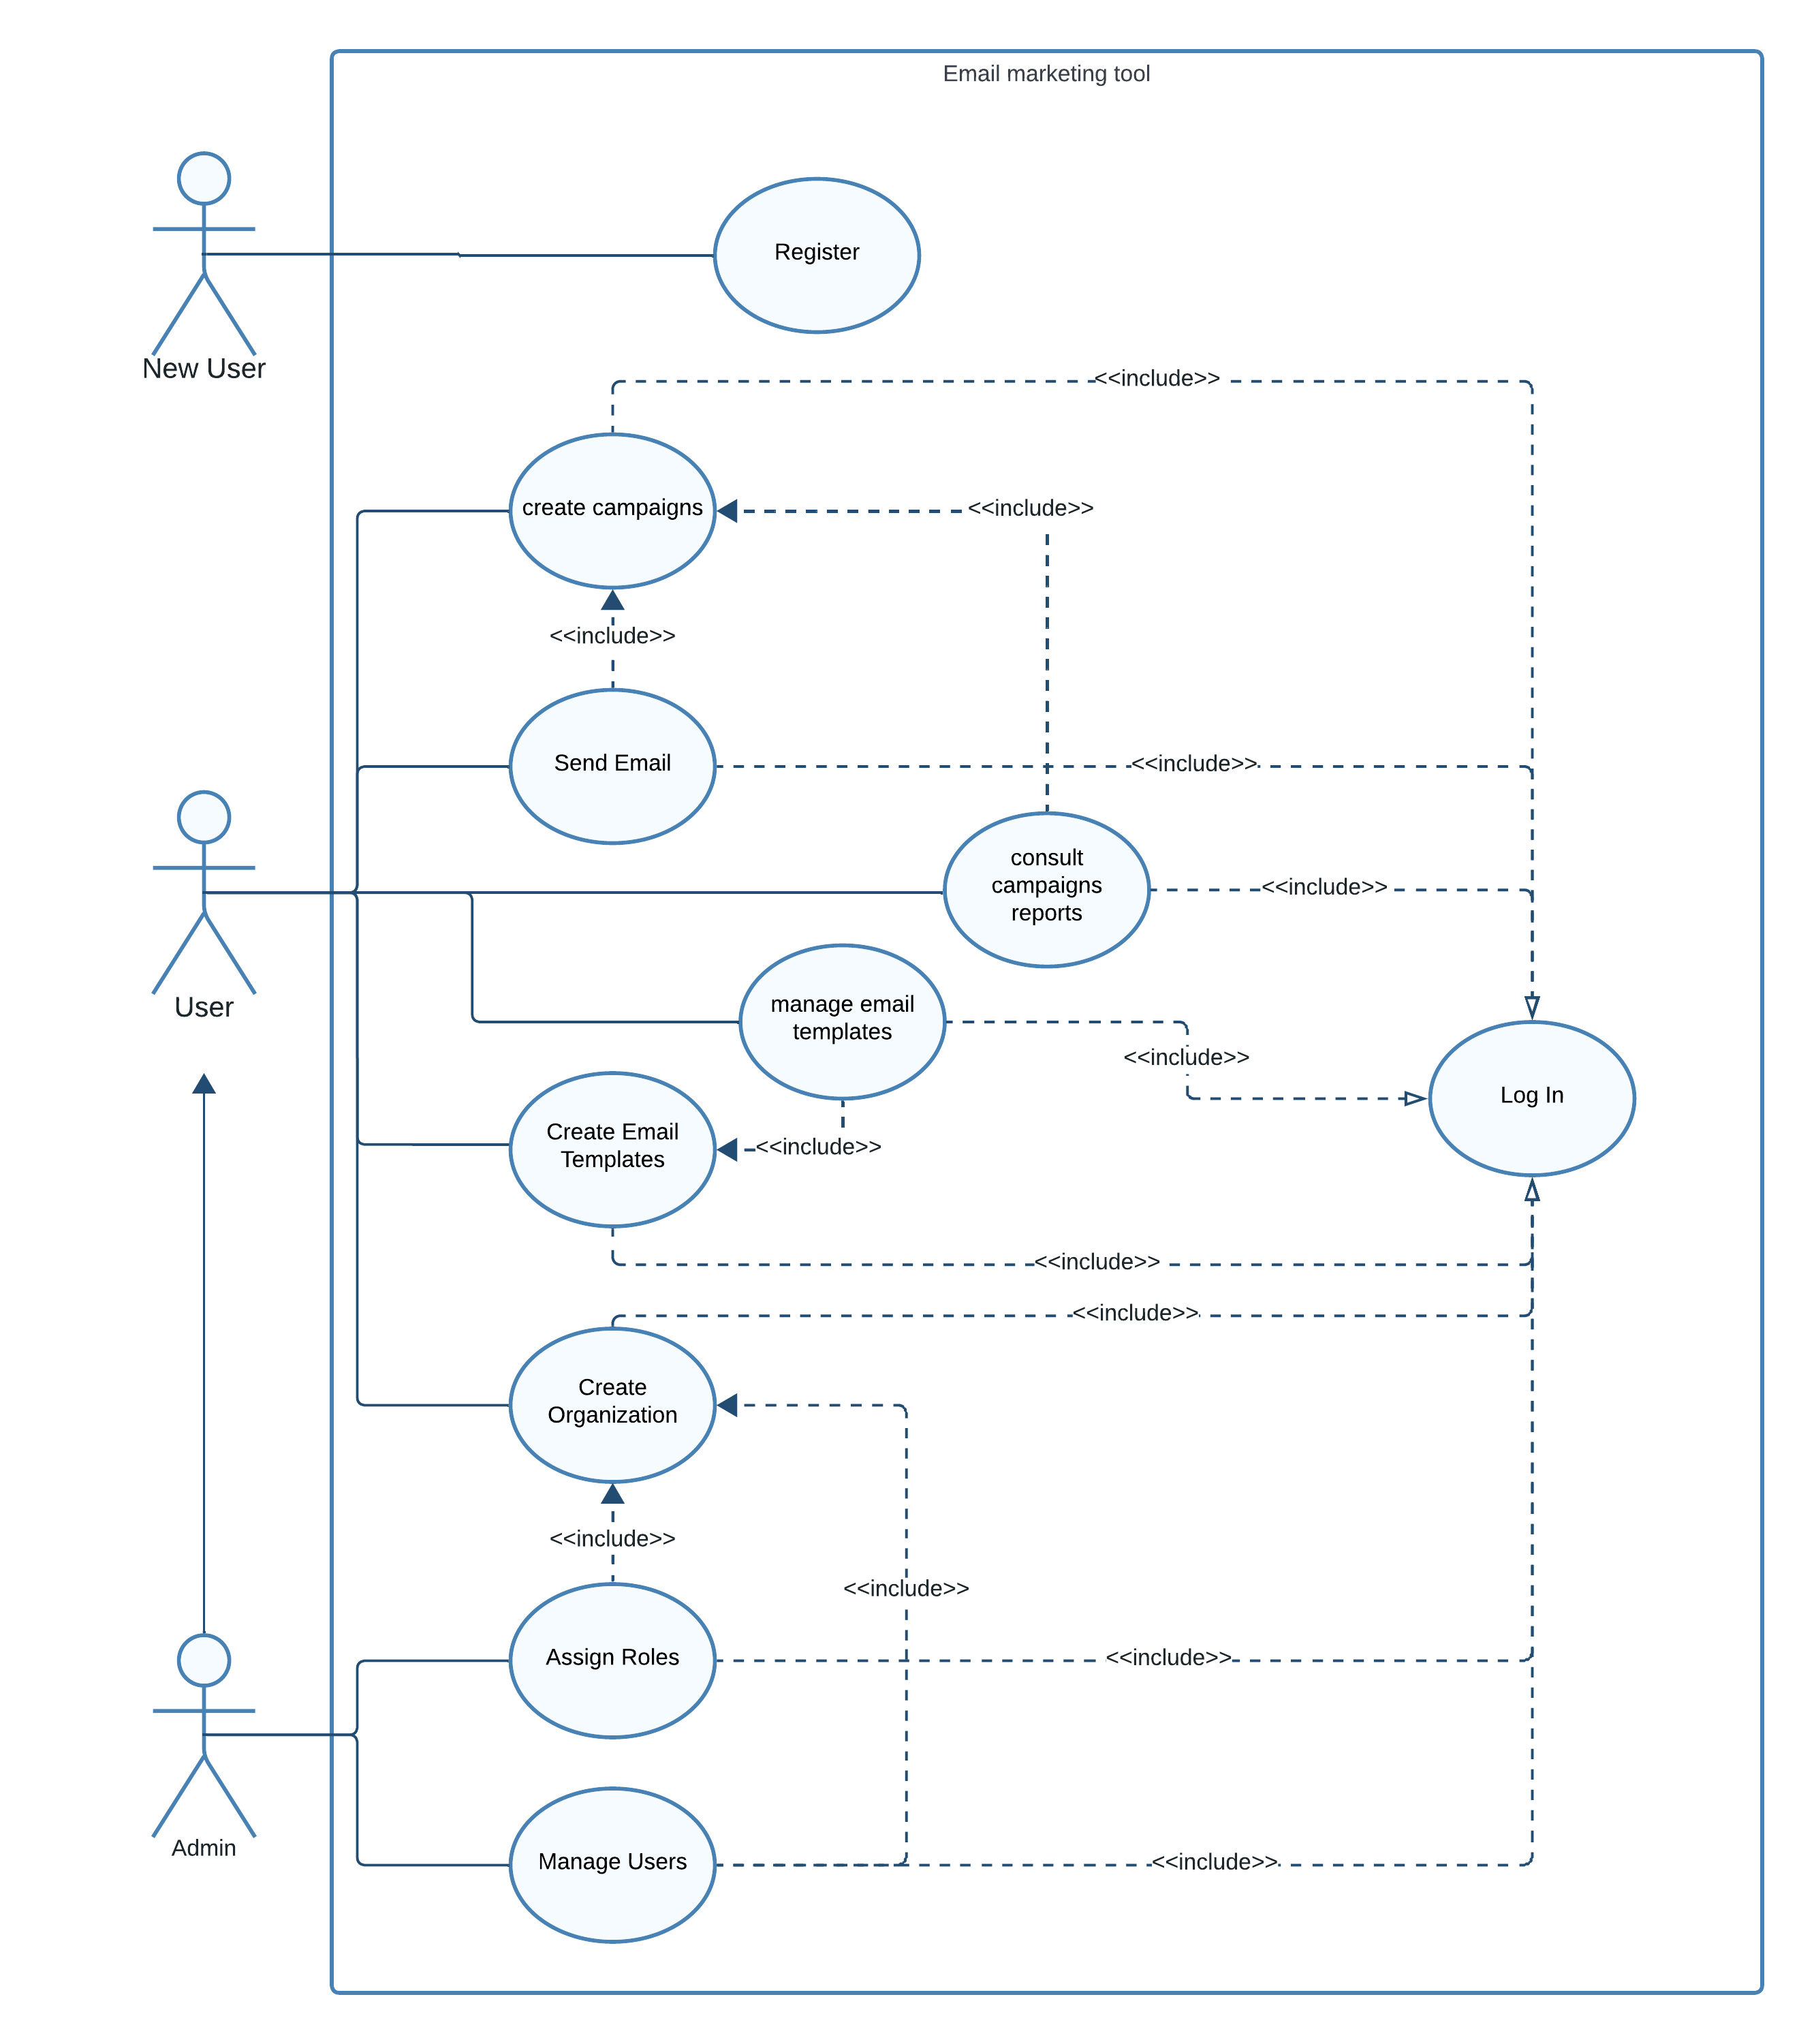
\includegraphics[width=\linewidth]{Images//images/global use case diag.png}
	\caption{Global Use Case Diagram}
	\label{fig:Global Use Case Diagram}
\end{figure}

\newpage

\subsection{Sprint Planning}

Figure 2.20 outlines our project's sprint planning. Each sprint had specific goals and durations. The initial phase was for learning the necessary tools. \textbf{Sprint 1} focused on building the email builder and enabling email sending. \textbf{Sprint 2} implemented CI/CD pipelines and deployed the application. \textbf{Sprint 3} worked on creating and managing campaigns and audience management. \textbf{Sprint 4} implemented email tracking functionality. \textbf{Sprint 5} managed media and organization, and conducted final testing and bug fixing across all features. This structured approach ensured thorough development and testing of each feature. As a result, all planned features were successfully implemented and thoroughly tested within the project timeline.

\begin{figure}[ht]
	\centering
	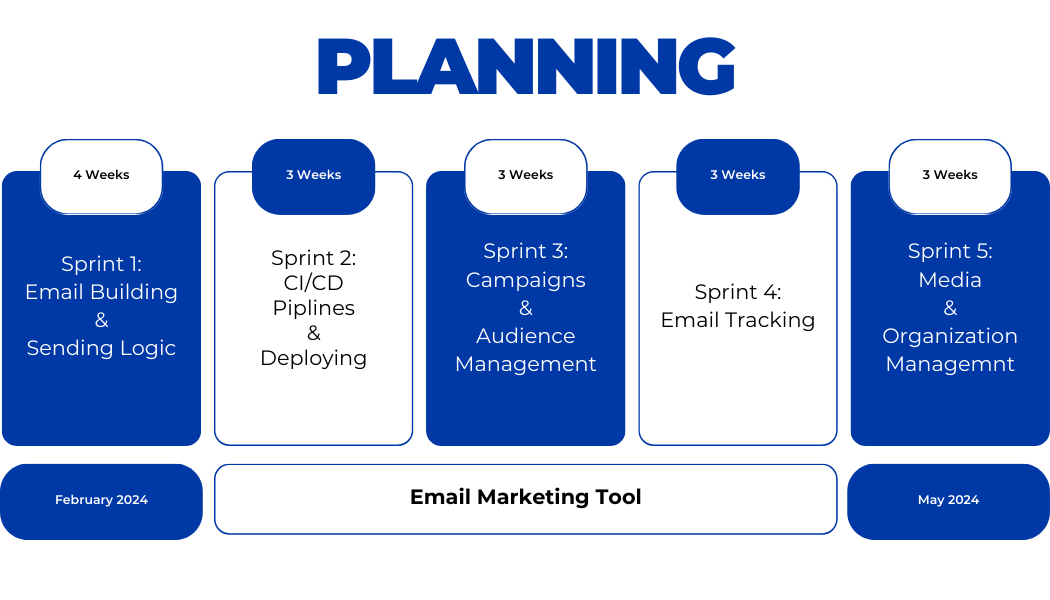
\includegraphics[width=\linewidth]{Images//images/planning.png}
	\caption{Sprint Planning}
	\label{fig:Sprint Planning}
\end{figure}
